\subsection{Linear Classifier}
The goal of linear classification is to take an input vector with multiple x values and assign it to one of multiple classes K. This can be done with one or more linear decision boundaries. The first way to classify is called the one-vs-one linear classifier. This works for 2 classes as seen in figure \ref{onevsone1}. If multiple clusters of x belonging to more than 2 classes are present we get ambiguous regions as one class might appear to be two different classes. An example of this can be seen in figure \ref{onevsone2}.
\begin{figure}[H]
\centering
\begin{minipage}[b]{0.5\textwidth}
\centering
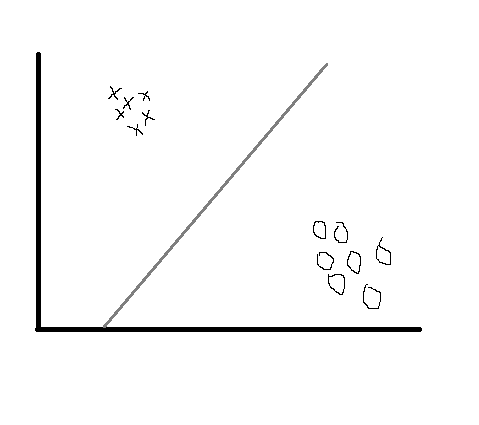
\includegraphics[scale=0.5]{billeder/onevsone1}
\caption{One-vs-one linear classifier for 2 classes}
\label{onevsone1}
\end{minipage}%
\begin{minipage}[b]{0.5\textwidth}
\centering
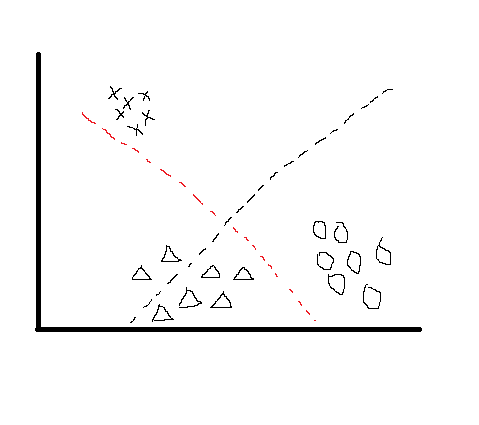
\includegraphics[scale=0.5]{billeder/onevsone2}
\caption{One-vs-one linear classifier for 3 classes}
\label{onevsone2}
\end{minipage}
\end{figure}
Another way to classify  the 3 classes seen in figure \ref{onevsone2} could be to utilise 1-of-k classification. This can be seen in figure \ref{oneofk1}. The 1-of-k classifier  has no ambiguity in this case.
\begin{figure}[H]
\centering
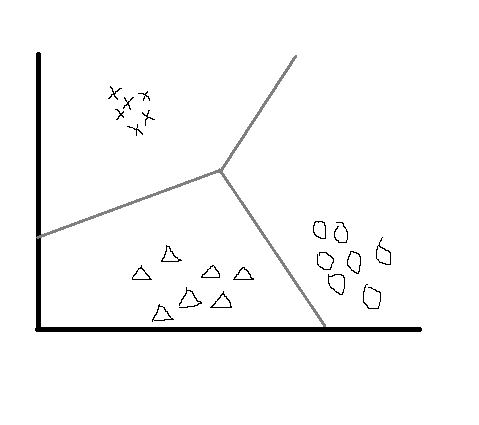
\includegraphics[scale=0.5]{billeder/oneofk1}
\caption{1-of-k linear classifier for 3 classes}
\label{oneofk1}
\end{figure}
In math terms the one-vs-one can be written as:
\begin{equation}
\label{oneofkcostfunc}
y(\textbf{x})=\tilde{\textbf{w}}^T\tilde{\textbf{x}}
\end{equation}
This is because we can consider the output y to be a weighted sum of the inputs. The error function can be defined as:
\begin{equation}
E(w) = \Sigma_n (\hat{y}(w,x_n) - y_n)^2
\end{equation}
Where $\hat{y}$ is the estimated $y$ value and $y_n$ is the true $y$ value.

If we look at a case with more than two classes, the linear classifier is prone to ambiguity. We know that the ambiguity issue can be avoid by using the form:
\begin{equation}
y_k(\textbf{x})=\textbf{w}_k^T\textbf{x}+\omega_{k0}
\end{equation}
and choosing the value of x to be a part of class k if $y_k(\textbf{x})>y_{m}(\textbf{x})$ for all $m \neq k$. This leads to decision boundaries corresponding to the 1-of-k classifier where the decision boundaries join together in the middle corresponding to the image in figure \ref{oneofk1}.\\\ \\


Training the one-of-k function requires the use of two vectors in matlab: $t$ and $Z$. t is vector of the correct classes while Z is a vector containing our features. In order to train the one-of-k classifier we use the following equation:
\begin{equation}
w^* = (Z^T Z)^{-1} Z^T t
\end{equation}
This results in the estimated weights for the classifier. To classify the data we use the cost function described earlier in equation \ref{oneofkcostfunc}.
In order to observe the boundaries in the project, the data must be 2 or 3 dimensional. This will require either the use of the PCA or fisher reduction methods explained in early sections. This leads to the image seen in figure \ref{2dimoneofk}.
\begin{figure}[H]
\centering
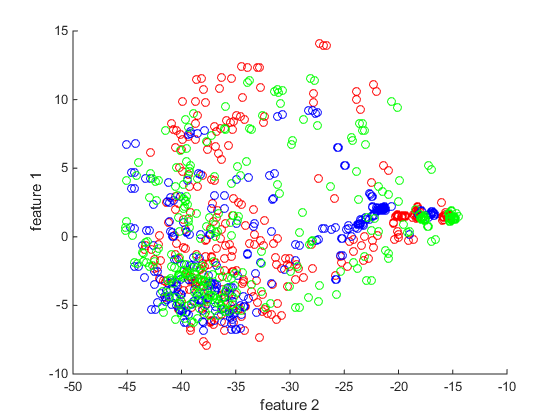
\includegraphics[scale=0.5]{billeder/2dimoneofk}
\caption{2 dimensional 1-of-k linear classifier for 3 classes of speech}
\label{2dimoneofk}
\end{figure}
This does not provide a usable visual representation of the classifier. The choice was made to keep the data in the higher dimensions.\\\ \\
The output from the cost function provides a sample and the values representing the three classes:
\begin{verbatim}
0.5333
0.2506
0.2160
\end{verbatim}
The highest value indicates that it belongs to this class. The cost function classifies the first sample to belong to class 1 as an example. The values from the cost function cannot be seen as a metric for how well it fits the class, just that it fits more the one class then the other. \\\ \\

The test data for each class was run through the cost function. This resulted in three plots as can be seen in figure \ref{fig:oneofkval1}, \ref{fig:oneofkval2} \& \ref{fig:oneofkval3}. The classes are coloured: Class 1 (Nicolai) = Red,  Class 2 (Rasmus) = Blue,  Class 3 (Rune) = Green.
\begin{figure}[H]
\minipage{0.32\textwidth}
  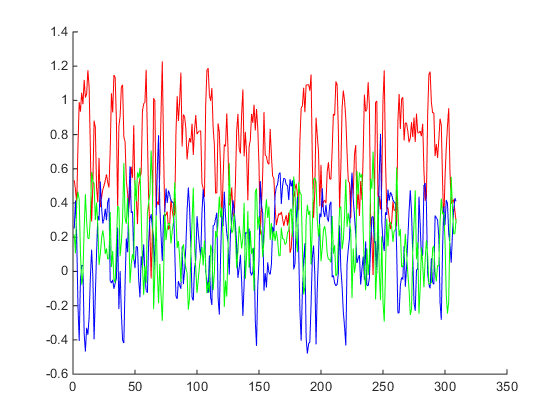
\includegraphics[width=\linewidth]{billeder/oneofkval1}
  \caption{Output from Nicolai data}\label{fig:oneofkval1}
\endminipage\hfill
\minipage{0.32\textwidth}
  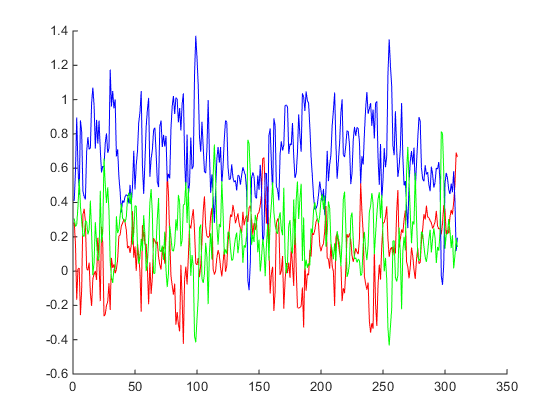
\includegraphics[width=\linewidth]{billeder/oneofkval2}
  \caption{Output from Rasmus data }\label{fig:oneofkval2}
\endminipage\hfill
\minipage{0.32\textwidth}%
  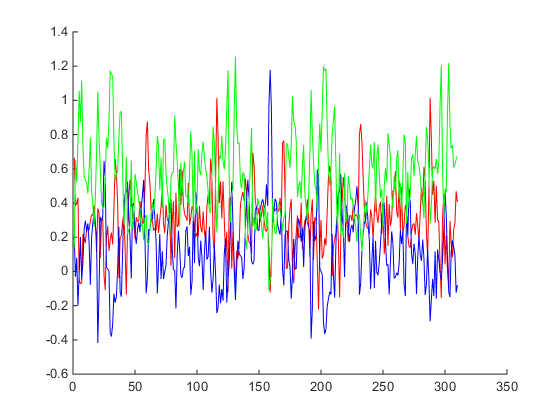
\includegraphics[width=\linewidth]{billeder/oneofkval3}
  \caption{Output from Rune data}\label{fig:oneofkval3}
\endminipage
\end{figure}
When evaluating the peak values of the three plots, it can be observed that the classifier correctly detriment that the first data set belongs to Nicolai, the second to Rasmus and the last to Rune. This can also be shown in a confusion matrix as seen on figure \ref{fig:conmatlin}: 

\begin{figure}[H]
\centering
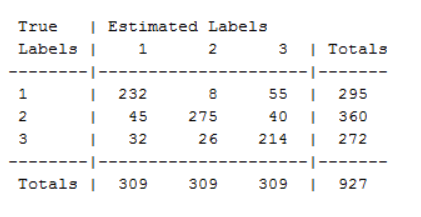
\includegraphics[scale=0.8]{billeder/conmatlin}
\caption{Confusion matrix for the linear model }
\label{fig:conmatlin}
\end{figure}

Here we see that the linear classifier can separate in the classes whit a error rate at 22.22\%. We see that Rune is the hardest to detect using this method, whit a 30.74\% error rate. 

%------------------------------------------------